% \documentclass[a4paper,10pt]{article}
% \usepackage[utf8]{inputenc}
% \usepackage{geometry}
% \usepackage{amsmath}
% \usepackage[table]{xcolor}
% \usepackage{colortbl}
% \usepackage{color,soul}
% \geometry{margin=0.8in}
% \usepackage{xcolor}
% \usepackage{tikz}
% \usetikzlibrary{matrix,fit,backgrounds}
% \usepackage{minted}
% \definecolor{bgcolor}{rgb}{0.8, 0.9, 0.5} % 
% \definecolor{bgcolor1}{rgb}{0.95, 0.95, 0.95} % Light Gray
% \definecolor{bgcolor2}{rgb}{0.85, 0.92, 1.0}  % Soft Blue
% \definecolor{bgcolor3}{rgb}{0.9, 0.85, 1.0}   % Light Purple
% \definecolor{bgcolor4}{rgb}{0.95, 0.88, 0.76} % Warm Beige
% \definecolor{bgcolor5}{rgb}{0.8, 0.95, 0.8}   % Gentle Green
% \definecolor{bgcolor6}{rgb}{1.0, 0.87, 0.87}  % Pastel Red
% \definecolor{bgcolor7}{rgb}{0.86, 0.93, 0.83} % Mint Green
% \definecolor{bgcolor8}{rgb}{0.98, 0.85, 0.94} % Soft Pink
% \definecolor{bgcolor9}{rgb}{0.87, 0.94, 0.98} % Sky Blue
% \definecolor{bgcolor10}{rgb}{0.96, 0.96, 0.82} % Pale Yellow
% 
% \begin{document}
\section*{Dynamic Programming Problem Codes}
% 1. Memoization
\subsection*{\textcolor{green}{\textbf{1. Memoization (Top-Down DP)}}}
\rule{\linewidth}{0.5mm}

We start with a recursive solution and use a 2D array \texttt{dp[i][j]} to store intermediate results to avoid recomputation.

\textbf{Recurrence:}
\[
dp[i][j] = \text{some function of }( dp[i-1][j], dp[i-1][j-1], \ldots)
\]
\begin{Verbatim}[fontsize=\small]
int dp[n][m];
int solve(int i, int j)
    if (base case) return value;
    if (dp[i][j] != -1) return dp[i][j];
    return dp[i][j] = f(solve(i-1, j), solve(i-1, j-1), ...);

\end{Verbatim}

% 2. Tabulation
\subsection*{\textcolor{red}{\textbf{2. Tabulation (Bottom-Up 2D DP)}}}
\rule{\linewidth}{0.5mm}

We convert the recursive structure into an iterative one by filling the \texttt{dp} table in a specific order.

\begin{Verbatim}[fontsize=\small]
for (int i = 0; i <= n; ++i) 
    for (int j = 0; j <= m; ++j) 
        if (base case) dp[i][j] = value;
        else dp[i][j] = f(dp[i-1][j], dp[i-1][j-1], ...);
\end{Verbatim}

% 3. 2-Row Optimization
\subsection*{\textcolor{orange}{\textbf{3. Space Optimization to 2 Rows}}}
\rule{\linewidth}{0.5mm}

Since each row only depends on the previous row, we can reduce space from \texttt{O(n*m)} to \texttt{O(2*m)}.

\begin{Verbatim}[fontsize=\small]
int prev[m+1], curr[m+1];
for (int i = 0; i <= n; ++i) 
    for (int j = 0; j <= m; ++j) 
        if (base case) curr[j] = value;
        else curr[j] = f(prev[j], prev[j-1], ...);
    
    swap(prev, curr);
\end{Verbatim}

% 4. 1-Row Optimization
\subsection*{\textcolor{yellow}{\textbf{4. Space Optimization to 1 Row}}}
\rule{\linewidth}{0.5mm}

If updates are done in reverse (right to left), we can reuse a single array.

\begin{Verbatim}[fontsize=\small]
int dp[m+1];
for (int i = 0; i <= n; ++i)
    for (int j = m; j >= 0; --j)
        if (base case) dp[j] = value;
        else dp[j] = f(dp[j], dp[j-1], ...);
    
\end{Verbatim}

% 5. Diagram
\subsection*{\textcolor{blue}{\textbf{5. Transition Diagram}}}
\rule{\linewidth}{0.5mm}

\begin{center}
\begin{tikzpicture}[node distance=2.5cm, every node/.style={draw, circle, fill=bgcolor5}, align=center]
\node (A) {Memoization\\(Top-Down)};
\node (B) [right of=A] {2D DP\\(Bottom-Up)};
\node (C) [right of=B] {2-Row DP};
\node (D) [right of=C] {1-Row DP};

\draw[->, thick] (A) -- (B) node[midway, above] {Tabulation};
\draw[->, thick] (B) -- (C) node[midway, above] {Space Opt.};
\draw[->, thick] (C) -- (D) node[midway, above] {Further Opt.};
\end{tikzpicture}
\end{center}

\noindent\textbf{Problem: Binomial Coefficient Pascal's Triangle C (n,k)= C(n-1,k-1) + C(n,k-1)}
\begin{minted}[
bgcolor=bgcolor2,
frame=lines,
framesep=5mm,
rulecolor=\color{black},
linenos,
numbersep=5pt,
fontsize=\normalsize
]{python}
""" MEMOIZATION : easy to implement using @lru_cache (from functools) or a manual dict"""
from functools import lru_cache

def binomial_coeff(n: int, k: int) -> int:
   
    @lru_cache(maxsize=None)  # Python built-in memoization
    def helper(n, k):
        # Base cases
        if k == 0 or k == n:
            return 1
        if k < 0 or k > n:
            return 0
        # Recursive case
        return helper(n - 1, k - 1) + helper(n - 1, k)
        
    return helper(n, k)
"""" MEMOIZATION : Manual dictionary Space Complexity (Same as above) : O(n * k) """
def binomial_coeff(n: int, k: int) -> int:
    memo = {}

    def helper(n, k):
        if k == 0 or k == n:
            return 1
        if k < 0 or k > n:
            return 0
        if (n, k) in memo:
            return memo[(n, k)]
        memo[(n, k)] = helper(n - 1, k - 1) + helper(n - 1, k)
        return memo[(n, k)]
    
    return helper(n, k)
"""Computes C(n, k) using bottom-up DP(tabulation).Space Complexity: O(n * k)"""
def binomial_coeff(n: int, k: int) -> int:
    # Initialize a (n+1) x (k+1) 2D table with zeros
    dp = [[0] * (k + 1) for _ in range(n + 1)]

    # Fill the table using base cases and recurrence
    for i in range(n + 1):
        for j in range(min(i, k) + 1):  # C(i, j) is 0 when j > i
            if j == 0 or j == i:
                dp[i][j] = 1  # Base cases
            else:
                dp[i][j] = dp[i - 1][j - 1] + dp[i - 1][j]

    return dp[n][k]
""" Computes C(n, k) using bottom-up DP with two rows.Space Complexity: O(2 * k)=O(k)"""
def binomial_coeff(n: int, k: int) -> int:
    prev = [0] * (k + 1)
    curr = [0] * (k + 1)
    
    prev[0] = 1  # Base case: C(0, 0) = 1

    for i in range(1, n + 1):
        curr[0] = 1  # C(i, 0) = 1 for all i
        for j in range(1, min(i, k) + 1):
            curr[j] = prev[j - 1] + prev[j]
        # Swap rows for the next iteration  (no need to copy)
        prev, curr = curr, prev
    
    return prev[k]
""" Computes C(n, k) using most efficient 1 row Tabulation DP Space Complexity: O(k)   """
def binomial_coeff(n: int, k: int) -> int:
    dp = [0] * (k + 1)
    dp[0] = 1  # Base case: C(0,0)=1
    
    # Build the Pascal's Triangle row-by-row
    for i in range(1, n + 1):
        # Update from right to left to avoid overwriting values we still need
        for j in range(min(i, k), 0, -1):
            dp[j] = dp[j] + dp[j - 1]
            # Equivalent to C(i, j) = C(i-1, j) + C(i-1, j-1)
    
    return dp[k]
\end{minted}

\noindent\textbf{Problem: Minimum Jumps to Reach End}
\begin{minted}[
bgcolor=bgcolor5,
frame=lines,
framesep=5mm,
rulecolor=\color{black},
linenos,
numbersep=5pt,
fontsize=\normalsize
]{python}
def min_jumps(arr: List[int]) -> int:
    """
    Finds minimum jumps to reach end of array.
    Time Complexity: O(n^2)       Space Complexity: O(n)
    """
    n = len(arr)
    if n <= 1:
        return 0
    jumps = [float('inf')] * n
    jumps[0] = 0
    
    for i in range(1, n):
        for j in range(i):
            if j + arr[j] >= i and jumps[j] != float('inf'):
                jumps[i] = min(jumps[i], jumps[j] + 1)
    
    return jumps[-1] if jumps[-1] != float('inf') else -1
\end{minted}
\begin{center}
\begin{tikzpicture}[scale=1.2, every node/.style={font=\small}]
    % Sequence of numbers
    \foreach \val/\x in {3/0, 10/1, 2/2, 1/3, 20/4, 4/5, 6/6, 7/7, 30/8} {
        \node[circle, draw=black, fill=bgcolor7, minimum size=8mm] (N\x) at (\x*1.2,0) {\val};
    }

    % Highlighted LIS: 3 → 4 → 6 → 7 → 30
    \foreach \from/\to in {0/5, 5/6, 6/7, 7/8} {
        \draw[->, thick, blue] (N\from) -- (N\to);
    }

    % Labels
    \node at (5.5, 1.2) {\textcolor{blue}{\textbf{Longest Increasing Subsequence}}};
    \node at (5.5, -1.2) {\texttt{LIS = [3, 4, 6, 7, 30]}};

\end{tikzpicture}
\end{center}

\noindent\textbf{Problem: Longest Increasing Subsequence (O(n²))}
\begin{minted}[
bgcolor=bgcolor4,
frame=lines,
framesep=5mm,
rulecolor=\color{black},
linenos,
numbersep=5pt,
fontsize=\normalsize
]{python}
def lis(nums: List[int]) -> int:
    """
    Finds length of longest increasing subsequence (O(n²)).
    Time Complexity: O(n^2)       Space Complexity: O(n)
    """
    n = len(nums)
    dp = [1] * n
    for i in range(1, n):
        for j in range(i):
            if nums[i] > nums[j]:
                dp[i] = max(dp[i], dp[j] + 1)
    return max(dp) if dp else 0
\end{minted}

\noindent\textbf{Problem: Longest Increasing Subsequence (O(n log n))}
\begin{minted}[
bgcolor=bgcolor7,
frame=lines,
framesep=5mm,
rulecolor=\color{black},
linenos,
numbersep=5pt,
fontsize=\normalsize
]{python}
import bisect

def lis_fast(nums: List[int]) -> int:
    """
    Finds length of longest increasing subsequence (O(n log n)).
    Time Complexity: O(n log n)       Space Complexity: O(n)
    """
    tails = []
    for num in nums:
        # Find position to maintain sorted order
        idx = bisect.bisect_left(tails, num)
        if idx == len(tails):
            tails.append(num)
        else:
            tails[idx] = num
    return len(tails)
\end{minted}

\noindent\textbf{Problem: Number of Longest Increasing Subsequences}
\begin{minted}[
bgcolor=bgcolor3,
frame=lines,
framesep=5mm,
rulecolor=\color{black},
linenos,
numbersep=5pt,
fontsize=\normalsize
]{python}
def find_number_of_lis(nums: List[int]) -> int:
    """
    Counts number of longest increasing subsequences.
    Time Complexity: O(n^2)       Space Complexity: O(n)
    """
    n = len(nums)
    if n <= 1: return n
    lengths = [1] * n  # Length of LIS ending at i
    counts = [1] * n   # Count of LIS ending at i
    
    for i in range(n):
        for j in range(i):
            if nums[i] > nums[j]:
                if lengths[j] + 1 > lengths[i]:
                    lengths[i] = lengths[j] + 1
                    counts[i] = counts[j]
                elif lengths[j] + 1 == lengths[i]:
                    counts[i] += counts[j]
    
    max_len = max(lengths)
    return sum(counts[i] for i in range(n) if lengths[i] == max_len)
\end{minted}
\noindent\textbf{Problem: Print All the  Longest Increasing Subsequences}
\begin{minted}[
bgcolor=bgcolor3,
frame=lines,
framesep=5mm,
rulecolor=\color{black},
linenos,
numbersep=5pt,
fontsize=\normalsize
]{python}
def print_all_lis(nums: List[int]) -> List[List[int]]:
"""     Time Complexity: O(n^2 + k*L) k: no of LIS       
        Space Complexity: O(n^2) + recursion stack
"""
    n = len(nums)
    if n == 0:
        return []

    # Phase 1: Compute LIS lengths
    dp = [1] * n
    prev = [[] for _ in range(n)]  # To store predecessors

    for i in range(n):
        for j in range(i):
            if nums[j] < nums[i]:
                if dp[j] + 1 > dp[i]:
                    dp[i] = dp[j] + 1
                    prev[i] = [j]
                elif dp[j] + 1 == dp[i]:
                    prev[i].append(j)

    max_len = max(dp)
    results = []

    # Phase 2: Backtrack to collect all sequences
    def dfs(i, path):
        if not prev[i]:
            if len(path) == max_len - 1:
                results.append([nums[i]] + path)
            return
        for j in prev[i]:
            dfs(j, [nums[i]] + path)

    for i in range(n):
        if dp[i] == max_len:
            dfs(i, [])

    return results
\end{minted}
\noindent\textbf{Problem: Maximum Number of Bridges without crossing}
\\
\begin{figure}[h!]
\centering
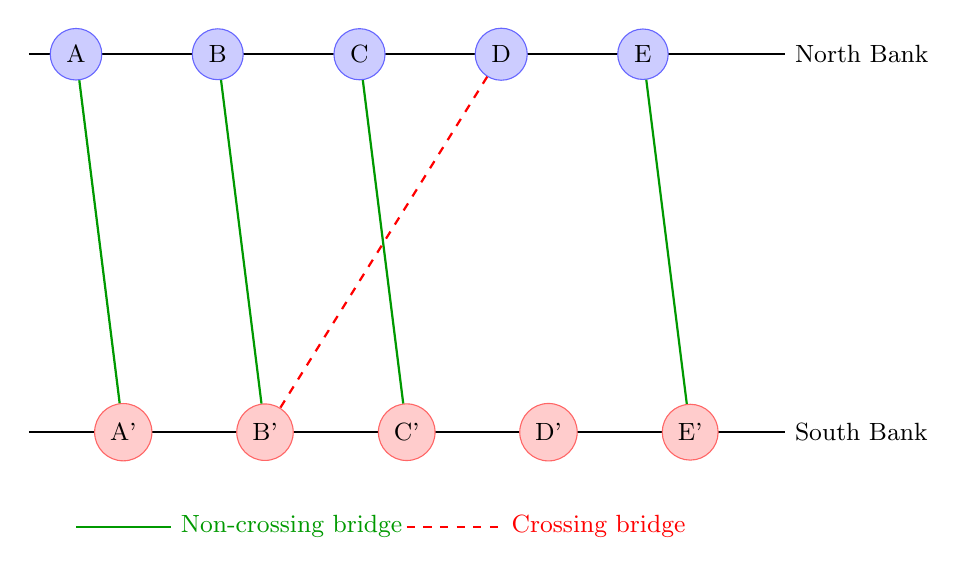
\begin{tikzpicture}[scale=1.2, every node/.style={font=\small}]
    % Draw banks
    \draw[thick] (0,0) -- (8,0) node[right] {South Bank};
    \draw[thick] (0,4) -- (8,4) node[right] {North Bank};

    % North bank cities
    \foreach \x/\name in {0.5/A, 2/B, 3.5/C, 5/D, 6.5/E} {
        \node[circle, draw=blue!60, fill=blue!20, minimum size=6mm] (N\name) at (\x,4) {\name};
    }

    % South bank cities
    \foreach \x/\name in {1/A', 2.5/B', 4/C', 5.5/D', 7/E'} {
        \node[circle, draw=red!60, fill=red!20, minimum size=6mm] (S\name) at (\x,0) {\name};
    }

    % Bridges (some crossing, some non-crossing)
    \draw[thick, green!60!black] (NA) -- (SA');
    \draw[thick, green!60!black] (NB) -- (SB');
    \draw[thick, green!60!black] (NC) -- (SC');
    \draw[thick, red, dashed] (ND) -- (SB'); % crossing
    \draw[thick, green!60!black] (NE) -- (SE');

    % Legend
    \draw[thick, green!60!black] (0.5,-1) -- (1.5,-1) node[right] {Non-crossing bridge};
    \draw[thick, red, dashed] (4,-1) -- (5,-1) node[right] {Crossing bridge};

\end{tikzpicture}
\caption{After sorting by north: [(1,2), (2,4), (3,3), (4,1)] - 
Now find LIS on south: [2, 4, 3, 1] - LIS is [2, 3] - answer is 2}
\end{figure}
\begin{minted}[
bgcolor=bgcolor1,
frame=lines,
framesep=5mm,
rulecolor=\color{black},
linenos,
numbersep=5pt,
fontsize=\normalsize
]{python}
def max_bridges(north: List[int], south: List[int]) -> int:
    """
    Finds the max number of non-crossing bridges.
    Time Complexity: O(n log n)
    """
    pairs = sorted(zip(north, south), key=lambda x: (x[0], x[1]))
    south_sorted = [s for _, s in pairs]

    # Find LIS on south_sorted
    import bisect
    lis = []
    for val in south_sorted:
        idx = bisect.bisect_left(lis, val)
        if idx == len(lis):
            lis.append(val)
        else:
            lis[idx] = val
    return len(lis)
\end{minted}
\noindent\textbf{Problem: 0-1 Knapsack}
\begin{minted}[
bgcolor=bgcolor,
frame=lines,
framesep=5mm,
rulecolor=\color{black},
linenos,
numbersep=5pt,
fontsize=\normalsize
]{python}
def knapSack(W: int, wt: List[int], val: List[int], n: int) -> int:
    """
    Solves 0-1 knapsack problem.
    Time Complexity: O(n*W)       Space Complexity: O(W)
    """
    dp = [0] * (W + 1)
    for i in range(1, n + 1):
        for w in range(W, 0, -1):
            if wt[i - 1] <= w:
                dp[w] = max(dp[w], dp[w - wt[i - 1]] + val[i - 1])
    return dp[W]
\end{minted}

\noindent\textbf{Problem: Subset Sum}
\begin{minted}[
bgcolor=bgcolor7,
frame=lines,
framesep=5mm,
rulecolor=\color{black},
linenos,
numbersep=5pt,
fontsize=\normalsize
]{python}
def subset_sum(nums, target):
    n = len(nums)
    dp = [[False] * (target + 1) for _ in range(n + 1)]
    
    # Base case: zero sum is always possible (empty subset)
    for i in range(n + 1):
        dp[i][0] = True

    for i in range(1, n + 1):
        for j in range(target + 1):
            if j < nums[i - 1]:
                dp[i][j] = dp[i - 1][j]
            else:
                dp[i][j] = dp[i - 1][j] or dp[i - 1][j - nums[i - 1]]

    return dp[n][target]

def subset_sum(nums: List[int], target: int) -> bool:
    """
    Checks if subset exists with given sum.
    Time Complexity: O(n*target)       Space Complexity: O(target)
    """
    dp = [False] * (target + 1)
    dp[0] = True
    for num in nums:
        for j in range(target, num - 1, -1):  # Update backwards
            dp[j] = dp[j] or dp[j - num]
    return dp[target]
\end{minted}

\noindent\textbf{Problem: Count of Subsets with Given Sum}
\begin{minted}[
bgcolor=bgcolor1,
frame=lines,
framesep=5mm,
rulecolor=\color{black},
linenos,
numbersep=5pt,
fontsize=\normalsize
]{python}
def count_subsets(nums: List[int], target: int) -> int:
    """
    Counts subsets with given sum.
    Time Complexity: O(n*target)       Space Complexity: O(target)
    """
    dp = [0] * (target + 1)
    dp[0] = 1
    for num in nums:
        for j in range(target, num - 1, -1):
            dp[j] += dp[j - num]
    return dp[target]
\end{minted}

\noindent\textbf{Problem: Minimum Subset Sum Difference}
\begin{minted}[
bgcolor=bgcolor9,
frame=lines,
framesep=5mm,
rulecolor=\color{black},
linenos,
numbersep=5pt,
fontsize=\normalsize
]{python}
def min_subset_diff(nums: List[int]) -> int:
    """
    Finds minimum difference between two subset sums.
    Time Complexity: O(n*sum)       Space Complexity: O(sum)
    """
    total = sum(nums)
    n = len(nums)
    dp = [False] * (total // 2 + 1)
    dp[0] = True
    
    for num in nums:
        # Update from right to left to avoid reuse of the same number
        for j in range(total // 2, num - 1, -1):
            if dp[j - num]:
                dp[j] = True

    # Find the largest j <= total//2 such that dp[j] is True
    for j in range(total // 2, -1, -1):
        if dp[j]:
            # Total - 2*j gives the minimum difference
            return total - 2 * j
    return float('inf')
\end{minted}

\noindent\textbf{Problem: Longest Common Subsequence}
\begin{center}
\begin{tikzpicture}[every node/.style={anchor=center, minimum size=8mm, font=\bfseries\large}]
    % Define the matrix
    \matrix (m) [matrix of nodes, nodes in empty cells,
        row sep=5mm, column sep=5mm,
        cells={draw, minimum width=6mm, minimum height=6mm}] {
        &   & A & B & C & D & E & F & G \\
        & 0 & 0 & 0 & 0 & 0 & 0 & 0 & 0 \\
      A & 0 & 1 & 1 & 1 & 1 & 1 & 1 & 1 \\
      E & 0 & 1 & 1 & 1 & 1 & 2 & 2 & 2 \\
      C & 0 & 1 & 1 & 2 & 2 & 2 & 2 & 2 \\
      F & 0 & 1 & 1 & 2 & 2 & 2 & 3 & 3 \\
      G & 0 & 1 & 1 & 2 & 2 & 2 & 3 & 4 \\
    };

    % Highlight LCS path: A → C → F → G
    \draw[very thick, green!70!black] (m-2-2.north west) -- (m-3-3.north west) -- (m-4-6.north west)
        -- (m-5-7.north west) -- (m-6-8.north west);

    % Label
    \node[below=1.5cm , text=green!50!black, font=\Huge\bfseries] {LCS = A, C, F, G};

\end{tikzpicture}
\end{center}
\begin{minted}[
bgcolor=bgcolor10,
frame=lines,
framesep=5mm,
rulecolor=\color{black},
linenos,
numbersep=5pt,
fontsize=\normalsize
]{python}
def lcs_length(text1: str, text2: str) -> int:
    m, n = len(text1), len(text2)
    dp = [[0] * (n + 1) for _ in range(m + 1)]

    for i in range(1, m + 1):
        for j in range(1, n + 1):
            if text1[i - 1] == text2[j - 1]:
                dp[i][j] = 1 + dp[i - 1][j - 1]
            else:
                dp[i][j] = max(dp[i - 1][j], dp[i][j - 1])

    return dp[m][n]

def lcs(X: str, Y: str) -> int:
    """
    Finds length of longest common subsequence.
    Time Complexity: O(m*n)       Space Complexity: O(min(m,n))
    """
    m, n = len(X), len(Y)
    if m < n:
        return lcs(Y, X)
    dp = [0] * (n + 1)
    for i in range(1, m + 1):
        prev = 0  # prev keeps track of dp[j-1] from the previous row (dp[i-1][j-1])
        for j in range(1, n + 1):
            temp = dp[j] # temp saves current dp[j] before it gets overwritten.
            if X[i - 1] == Y[j - 1]:
                dp[j] = prev + 1 # LCS between X[0..i-1] and Y[0..j-1]
            else:
                dp[j] = max(dp[j], dp[j - 1]) #dp[j] → value from the previous row (same j) 
                # and dp[j-1] → value to the left in current row
            prev = temp
    return dp[n]
\end{minted}

\noindent\textbf{Problem: Printing LCS}
\begin{minted}[
bgcolor=bgcolor5,
frame=lines,
framesep=5mm,
rulecolor=\color{black},
linenos,
numbersep=5pt,
fontsize=\normalsize
]{python}
def print_lcs(X: str, Y: str) -> str:
    """
    Prints longest common subsequence.
    Time Complexity: O(m*n)       Space Complexity: O(m*n)
    """
    m, n = len(X), len(Y)
    dp = [[0] * (n + 1) for _ in range(m + 1)]
    
    # Build DP table
    for i in range(1, m + 1):
        for j in range(1, n + 1):
            if X[i - 1] == Y[j - 1]:
                dp[i][j] = dp[i - 1][j - 1] + 1
            else:
                dp[i][j] = max(dp[i - 1][j], dp[i][j - 1])
    
    # Backtrack to find LCS
    res = []
    i, j = m, n
    while i > 0 and j > 0:
        if X[i - 1] == Y[j - 1]:
            res.append(X[i - 1])
            i -= 1
            j -= 1
        elif dp[i - 1][j] > dp[i][j - 1]:
            i -= 1
        else:
            j -= 1
    return ''.join(reversed(res))
\end{minted}
\noindent\textbf{Problem: Print SCS (Shortest Common Supersequence)}
\begin{minted}[
bgcolor=bgcolor4,
frame=lines,
framesep=5mm,
rulecolor=\color{black},
linenos,
numbersep=5pt,
fontsize=\normalsize
]{python}
def print_scs(X: str, Y: str) -> str:
    """
    Prints shortest common supersequence of two strings.
    Time Complexity: O(m*n)       Space Complexity: O(m*n)
    """
    m, n = len(X), len(Y)
    dp = [[0]*(n+1) for _ in range(m+1)]
    
    # Build LCS table
    for i in range(1, m+1):
        for j in range(1, n+1):
            if X[i-1] == Y[j-1]:
                dp[i][j] = 1 + dp[i-1][j-1]
            else:
                dp[i][j] = max(dp[i-1][j], dp[i][j-1])
    
    # Backtrack to construct SCS
    res = []
    i, j = m, n
    while i > 0 and j > 0:
        if X[i-1] == Y[j-1]:
            res.append(X[i-1])
            i -= 1
            j -= 1
        elif dp[i-1][j] > dp[i][j-1]:
            res.append(X[i-1])
            i -= 1
        else:
            res.append(Y[j-1])
            j -= 1
    
    # Add remaining characters
    while i > 0:
        res.append(X[i-1])
        i -= 1
    while j > 0:
        res.append(Y[j-1])
        j -= 1
        
    return ''.join(reversed(res))
\end{minted}

\noindent\textbf{Problem: Longest Repeating Subsequence}
\begin{minted}[
bgcolor=bgcolor9,
frame=lines,
framesep=5mm,
rulecolor=\color{black},
linenos,
numbersep=5pt,
fontsize=\normalsize
]{python}
def lrs(s: str) -> int:
    """
    Finds length of longest repeating subsequence.
    Time Complexity: O(n^2)       Space Complexity: O(n^2)
    """
    n = len(s)
    dp = [[0]*(n+1) for _ in range(n+1)]
    
    for i in range(1, n+1):
        for j in range(1, n+1):
            if s[i-1] == s[j-1] and i != j:
                dp[i][j] = 1 + dp[i-1][j-1]
            else:
                dp[i][j] = max(dp[i-1][j], dp[i][j-1])
    return dp[n][n]
\end{minted}

\noindent\textbf{Problem: Longest Repeating Substring (DP) (Also in Binary Search)}
\begin{minted}[
bgcolor=bgcolor8,
frame=lines,
framesep=5mm,
rulecolor=\color{black},
linenos,
numbersep=5pt,
fontsize=\normalsize
]{python}
def lrs_substring(s: str) -> int:
    """
    Finds length of longest repeating substring using DP.
    Time Complexity: O(n^2)       Space Complexity: O(n^2)
    """
    n = len(s)
    dp = [[0]*(n+1) for _ in range(n+1)]
    max_len = 0
    
    for i in range(1, n+1):
        for j in range(1, n+1):
            if s[i-1] == s[j-1] and i != j:
                dp[i][j] = 1 + dp[i-1][j-1]
                max_len = max(max_len, dp[i][j])
            else:
                dp[i][j] = 0
    return max_len
\end{minted}

\noindent\textbf{Problem: Length of Largest Subsequence of A which is Substring in B}
\begin{minted}[
bgcolor=bgcolor3,
frame=lines,
framesep=5mm,
rulecolor=\color{black},
linenos,
numbersep=5pt,
fontsize=\normalsize
]{python}
def max_common_subsequence_substring(A: str, B: str) -> int:
    """
    Finds largest subsequence of A that is substring in B.
    Time Complexity: O(m*n)       Space Complexity: O(n)
    """
    m, n = len(A), len(B)
    max_len = 0
    # dp[j] stores max length ending at j in B
    dp = [0] * (n+1)
    
    for i in range(1, m+1):
        # Traverse backwards to avoid overwriting
        for j in range(n, 0, -1):
            if A[i-1] == B[j-1]:
                dp[j] = 1 + dp[j-1]
                max_len = max(max_len, dp[j])
            else:
                dp[j] = 0  # Reset since it must be substring
    return max_len
\end{minted}

\noindent\textbf{Problem: Subsequence Pattern Matching}
\begin{minted}[
bgcolor=bgcolor,
frame=lines,
framesep=5mm,
rulecolor=\color{black},
linenos,
numbersep=5pt,
fontsize=\normalsize
]{python}
def is_subsequence(a: str, b: str) -> bool:
    """
    Checks if a is subsequence of b.
    Time Complexity: O(n)       Space Complexity: O(1)
    """
    i, j = 0, 0
    while i < len(a) and j < len(b):
        if a[i] == b[j]:
            i += 1
        j += 1
    return i == len(a)
\end{minted}

\noindent\textbf{Problem: Count of Subsequences of a in b}
\begin{minted}[
bgcolor=bgcolor8,
frame=lines,
framesep=5mm,
rulecolor=\color{black},
linenos,
numbersep=5pt,
fontsize=\normalsize
]{python}
def count_subsequences_recursive(a: str, b: str, m: int, n: int) -> int:

    # Base Case: If a is fully traversed, we found a subsequence match
    if m == 0:
        return 1

    # Base Case: If b is fully traversed but a is not, no more matches are possible
    if n == 0:
        return 0

    # If last characters match, we can either include it or skip it
    if a[m - 1] == b[n - 1]:
        # Include the matching character + skip the character
        return (count_subsequences_recursive(a, b, m - 1, n - 1) +
                count_subsequences_recursive(a, b, m, n - 1))
    else:
        # If characters don’t match, skip current character of b
        return count_subsequences_recursive(a, b, m, n - 1)
        
def count_subsequences(a: str, b: str) -> int:
    """
    Counts occurrences of a as subsequence in b.
    Time Complexity: O(m*n)       Space Complexity: O(m)
    """
    m, n = len(a), len(b)
    dp = [0] * (m+1)
    dp[0] = 1  # Empty string has 1 match
    
    for j in range(1, n+1):
        # Traverse backwards to avoid overwriting
        for i in range(m, 0, -1):
            if a[i-1] == b[j-1]:
                dp[i] += dp[i-1]
    return dp[m]
\end{minted}

\noindent\textbf{Problem: Longest Palindromic Substring}
\begin{minted}[
bgcolor=bgcolor7,
frame=lines,
framesep=5mm,
rulecolor=\color{black},
linenos,
numbersep=5pt,
fontsize=\normalsize
]{python}
def longest_palindromic_substring(s: str) -> str:
    """
    Finds longest palindromic substring using DP.
    Time Complexity: O(n^2)       Space Complexity: O(n^2)
    """
    n = len(s)
    dp = [[False]*n for _ in range(n)]
    start, max_len = 0, 1
    
    # All substrings of length 1 are palindromes
    for i in range(n):
        dp[i][i] = True
    
    # Check for length 2
    for i in range(n-1):
        if s[i] == s[i+1]:
            dp[i][i+1] = True
            start = i
            max_len = 2
    
    # Check lengths > 2
    for length in range(3, n+1):
        for i in range(n-length+1):
            j = i+length-1
            if s[i] == s[j] and dp[i+1][j-1]:
                dp[i][j] = True
                if length > max_len:
                    start = i
                    max_len = length
    return s[start:start+max_len]
\end{minted}

\noindent\textbf{Problem: Count of Palindromic Substrings}
\begin{minted}[
bgcolor=bgcolor4,
frame=lines,
framesep=5mm,
rulecolor=\color{black},
linenos,
numbersep=5pt,
fontsize=\normalsize
]{python}
def count_palindromic_substrings(s: str) -> int:
    """
    Counts all palindromic substrings in a string.
    Time Complexity: O(n^2)       Space Complexity: O(n^2)
    """
    n = len(s)
    dp = [[False]*n for _ in range(n)]
    count = 0
    
    for i in range(n):
        dp[i][i] = True
        count += 1
    
    for i in range(n-1):
        if s[i] == s[i+1]:
            dp[i][i+1] = True
            count += 1
    
    for length in range(3, n+1):
        for i in range(n-length+1):
            j = i+length-1
            if s[i] == s[j] and dp[i+1][j-1]:
                dp[i][j] = True
                count += 1
    return count
\end{minted}

\noindent\textbf{Problem: Minimum Insertions to Make Palindrome}
\begin{minted}[
bgcolor=bgcolor3,
frame=lines,
framesep=5mm,
rulecolor=\color{black},
linenos,
numbersep=5pt,
fontsize=\normalsize
]{python}
def min_insertions_recursive(s: str, i: int, j: int) -> int:
    # Base Case: If the substring has 0 or 1 character, it's already a palindrome
    if i >= j:
        return 0

    # If characters match, we can skip both ends
    if s[i] == s[j]:
        return min_insertions_recursive(s, i + 1, j - 1)
    else:
        # If they don't match, insert a character at either end
        # and solve the smaller subproblems, taking the minimal path
        insert_left = min_insertions_recursive(s, i + 1, j)
        insert_right = min_insertions_recursive(s, i, j - 1)
        return 1 + min(insert_left, insert_right)
def min_insertions_palindrome(s: str) -> int:
    """
    Finds minimum insertions to make string palindrome.
    Time Complexity: O(n^2)       Space Complexity: O(n^2)
    """
    n = len(s)
    dp = [[0]*n for _ in range(n)]
    
    for length in range(2, n+1):
        for i in range(n-length+1):
            j = i+length-1
            if s[i] == s[j]:
                dp[i][j] = dp[i+1][j-1]
            else: # characters don't match, insert on either side
                dp[i][j] = 1 + min(dp[i+1][j], dp[i][j-1])
    return dp[0][n-1]
\end{minted}

\noindent\textbf{Problem: Edit Distance}
\begin{minted}[
bgcolor=bgcolor2,
frame=lines,
framesep=5mm,
rulecolor=\color{black},
linenos,
numbersep=5pt,
fontsize=\normalsize
]{python}
def edit_distance(word1: str, word2: str) -> int:
    """
    Computes minimum edit operations (insert, delete, replace) to convert word1 to word2.
    Time Complexity: O(m*n)       Space Complexity: O(min(m,n))
    """
    m, n = len(word1), len(word2)
    if m < n:
        return edit_distance(word2, word1)
    
    dp = [0] * (n+1)
    # Initialize first row
    for j in range(n+1):
        dp[j] = j
    
    for i in range(1, m+1):
        prev = dp[0]
        dp[0] = i
        for j in range(1, n+1):
            temp = dp[j]
            if word1[i-1] == word2[j-1]:
                dp[j] = prev
            else:
                dp[j] = 1 + min(prev, dp[j], dp[j-1])
            prev = temp
    return dp[n]
\end{minted}
\noindent\textbf{Problem: Optimal Strategy for Game}
\begin{minted}[
bgcolor=bgcolor1,
frame=lines,
framesep=5mm,
rulecolor=\color{black},
linenos,
numbersep=5pt,
fontsize=\normalsize
]{python}
def optimal_strategy(arr: List[int]) -> int:
    """
    Maximizes value by choosing ends optimally (picking game).
    Time Complexity: O(n^2)       Space Complexity: O(n^2)
    """
    n = len(arr)
    dp = [[0]*n for _ in range(n)]
    
    for gap in range(n):
        for i in range(n - gap):
            j = i + gap
            x = dp[i+2][j] if i+2 <= j else 0
            y = dp[i+1][j-1] if i+1 <= j-1 else 0
            z = dp[i][j-2] if i <= j-2 else 0
            dp[i][j] = max(arr[i] + min(x, y), arr[j] + min(y, z))
    
    return dp[0][n-1]
\end{minted}

\noindent\textbf{Problem: Count BSTs with n Keys (Catalan Number)}
\begin{minted}[
bgcolor=bgcolor8,
frame=lines,
framesep=5mm,
rulecolor=\color{black},
linenos,
numbersep=5pt,
fontsize=\normalsize
]{python}
def count_bsts(n: int) -> int:
    """
    Counts structurally unique BSTs with n keys (Catalan number).
    Time Complexity: O(n^2)       Space Complexity: O(n)
    """
    dp = [0]*(n+1)
    dp[0] = 1
    for i in range(1, n+1):
        for j in range(i):
            dp[i] += dp[j] * dp[i-j-1]
    return dp[n]
\end{minted}

\noindent\textbf{Problem: Max Sum with No Adjacent Elements}
\begin{minted}[
bgcolor=bgcolor5,
frame=lines,
framesep=5mm,
rulecolor=\color{black},
linenos,
numbersep=5pt,
fontsize=\normalsize
]{python}
def max_sum_non_adjacent(arr: List[int]) -> int:
    """
    Finds maximum sum of non-adjacent elements.
    Time Complexity: O(n)       Space Complexity: O(1)
    """
    incl = 0
    excl = 0
    for num in arr:
        new_incl = excl + num
        excl = max(incl, excl)
        incl = new_incl
    return max(incl, excl)
\end{minted}
\noindent\textbf{Problem: Unbounded Knapsack}
\begin{minted}[
bgcolor=bgcolor10,
frame=lines,
framesep=5mm,
rulecolor=\color{black},
linenos,
numbersep=5pt,
fontsize=\normalsize
]{python}
def unbounded_knapsack_recursive(wt: list, val: list, W: int, n: int) -> int:
    # Base Case: No capacity or no items left
    if W == 0 or n == 0:
        return 0

    # If item can be included
    if wt[n - 1] <= W:
        # Include item (stay at same index to allow repetition)
        include = val[n - 1] + unbounded_knapsack_recursive(wt, val, W - wt[n - 1], n)
        # Exclude item (move to next index)
        exclude = unbounded_knapsack_recursive(wt, val, W, n - 1)
        return max(include, exclude)
    else:
        # Skip item if it can't fit
        return unbounded_knapsack_recursive(wt, val, W, n - 1)
def unbounded_knapsack_by_loop(wt: list, val: list, W: int) -> int:
    # Base case: no capacity left
    if W == 0:
        return 0

    max_val = 0
    # Try every item that fits in the current capacity
    for i in range(len(wt)):
        if wt[i] <= W:
            # Include item i and recur for reduced capacity W - wt[i]
            current = val[i] + unbounded_knapsack_by_loop(wt, val, W - wt[i])
            max_val = max(max_val, current)

    return max_val
def unbounded_knapsack(wt: list, val: list, W: int) -> int:
    n = len(wt)
    # Initialize DP table: dp[i][j] = max value using first i items for capacity j
    dp = [[0] * (W + 1) for _ in range(n + 1)]

    for i in range(1, n + 1):
        for j in range(W + 1):
            if wt[i - 1] <= j:
                # Include or exclude current item (can reuse)
                dp[i][j] = max(dp[i - 1][j], val[i - 1] + dp[i][j - wt[i - 1]])
            else:
                dp[i][j] = dp[i - 1][j]

    return dp[n][W]
def unbounded_knapsack(W: int, wt: List[int], val: List[int]) -> int:
    """
    Solves unbounded knapsack (multiple copies allowed).
    Time Complexity: O(n*W)       Space Complexity: O(W)
    """
    dp = [0]*(W+1)
    for w in range(1, W+1):
        for i in range(len(wt)):
            if wt[i] <= w:
                dp[w] = max(dp[w], dp[w - wt[i]] + val[i])
    return dp[W]
\end{minted}

\noindent\textbf{Problem: Rod Cutting Problem}
\begin{minted}[
bgcolor=bgcolor2,
frame=lines,
framesep=5mm,
rulecolor=\color{black},
linenos,
numbersep=5pt,
fontsize=\normalsize
]{python}
def rod_cutting_recursive(prices: list, n: int) -> int:
    # Base case: no length means no profit
    if n == 0:
        return 0

    max_profit = float('-inf')

    # Try every possible first cut from 1 to n
    for i in range(1, n + 1):
        # prices[i-1] is the price for rod length i
        profit = prices[i - 1] + rod_cutting_recursive(prices, n - i)
        max_profit = max(max_profit, profit)

    return max_profit

def rod_cutting(prices: List[int], n: int) -> int:
    """
    Maximizes profit by cutting rod optimally.
    Time Complexity: O(n^2)       Space Complexity: O(n)
    """
    dp = [0]*(n+1)
    for i in range(1, n+1):
        max_val = float('-inf')
        for j in range(i):
            max_val = max(max_val, prices[j] + dp[i-j-1])
        dp[i] = max_val
    return dp[n]
\end{minted}

\noindent\textbf{Problem: Coin Change (Total Ways)}
\begin{minted}[
bgcolor=bgcolor9,
frame=lines,
framesep=5mm,
rulecolor=\color{black},
linenos,
numbersep=5pt,
fontsize=\normalsize
]{python}
def coin_change_ways(coins: list, n: int, amount: int) -> int:
    # Base Case: If amount is 0, there's one valid way (choose nothing)
    if amount == 0:
        return 1

    # Base Case: If no coins left and amount not 0, no valid way
    if n == 0 and amount > 0:
        return 0

    # If current coin can be used
    if coins[n - 1] <= amount:
        # 1. Include coin[n-1] and stay at same index (unbounded)
        # 2. Exclude coin[n-1] and move to next
        return (coin_change_ways(coins, n, amount - coins[n - 1]) +
                coin_change_ways(coins, n - 1, amount))
    else:
        # Only option: exclude coin[n-1]
        return coin_change_ways(coins, n - 1, amount)
def coin_change_ways(coins: List[int],amount: int) ->int:
    n = len(coins)

    # dp[i][j] = ways to make amount j using first i coins
    dp = [[0] * (amount + 1) for _ in range(n + 1)]

    # Base case: 1 way to form amount 0 (choose nothing)
    for i in range(n + 1):
        dp[i][0] = 1

    # Fill the table row by row
    for i in range(1, n + 1):
        for j in range(amount + 1):
            # Exclude coin[i-1]
            dp[i][j] = dp[i - 1][j]
            # Include coin[i-1] if it fits
            if coins[i - 1] <= j:
                dp[i][j] += dp[i][j - coins[i - 1]]

    return dp[n][amount]
def coin_change_ways(coins: List[int], amount: int) -> int:
    """
    Counts ways to make amount using coins (order matters).
    Time Complexity: O(amount*n)       Space Complexity: O(amount)
    """
    dp = [0]*(amount+1)
    dp[0] = 1
    for coin in coins:
        for j in range(coin, amount+1):
            dp[j] += dp[j - coin] # same as above in consize way
    return dp[amount]
\end{minted}

\noindent\textbf{Problem: Maximum Cuts}
\begin{minted}[
bgcolor=bgcolor3,
frame=lines,
framesep=5mm,
rulecolor=\color{black},
linenos,
numbersep=5pt,
fontsize=\normalsize
]{python}
def max_cuts(n: int, a: int, b: int, c: int) -> int:
    """
    Maximizes cuts of length a, b, c in rod of length n.
    Time Complexity: O(n)       Space Complexity: O(n)
    """
    dp = [-10**9]*(n+1)
    dp[0] = 0
    for i in range(1, n+1):
        if i >= a: dp[i] = max(dp[i], dp[i-a] + 1)
        if i >= b: dp[i] = max(dp[i], dp[i-b] + 1)
        if i >= c: dp[i] = max(dp[i], dp[i-c] + 1)
    return dp[n] if dp[n] >= 0 else -1
\end{minted}

\noindent\textbf{Problem: Minimum Coins to Make Value}
\begin{minted}[
bgcolor=bgcolor4,
frame=lines,
framesep=5mm,
rulecolor=\color{black},
linenos,
numbersep=5pt,
fontsize=\normalsize
]{python}
def min_coins(coins: List[int], amount: int) -> int:
    """
    Finds minimum coins to make amount (inf supply).
    Time Complexity: O(amount*n)       Space Complexity: O(amount)
    """
    dp = [10**9]*(amount+1)
    dp[0] = 0
    for coin in coins:
        for j in range(coin, amount+1):
            dp[j] = min(dp[j], dp[j-coin] + 1)
    return dp[amount] if dp[amount] != 10**9 else -1
\end{minted}

\noindent\textbf{Problem: Buy \& Sell Stock II (Infinite Tx)}
\begin{minted}[
bgcolor=bgcolor7,
frame=lines,
framesep=5mm,
rulecolor=\color{black},
linenos,
numbersep=5pt,
fontsize=\normalsize
]{python}
def get_maximum_profit(prices: List[int]) -> int:
    n = len(prices)
    # dp[ind][buy] = max profit starting at day ind with buy-flag buy
    dp: List[List[int]] = [[-1, -1] for _ in range(n)]
    
    def get_ans(ind: int, buy: int) -> int:
        # Base case: no more days left
        if ind == n:
            return 0
        
        # Return cached result if available
        if dp[ind][buy] != -1:
            return dp[ind][buy]
        
        if buy == 0:
            # Option 1: skip buying today
            skip = get_ans(ind + 1, 0)
            # Option 2: buy today (subtract price), switch to sell-mode
            buy_stock = -prices[ind] + get_ans(ind + 1, 1)
            profit = max(skip, buy_stock)
        else:
            # Option 1: skip selling today
            skip = get_ans(ind + 1, 1)
            # Option 2: sell today (add price), switch to buy-mode
            sell_stock = prices[ind] + get_ans(ind + 1, 0)
            profit = max(skip, sell_stock)
        
        dp[ind][buy] = profit
        return profit
    
    # Start at day 0 with ability to buy
    return get_ans(0, 0)
from typing import List

def max_profit_tabulation(prices: List[int]) -> int:
    """
    Bottom-up 2D DP for unlimited transactions.
    
    dp[ind][0] = max profit from day ind if we can BUY
    dp[ind][1] = max profit from day ind if we can SELL
    """
    n = len(prices)
    # Create dp table with one extra row for the base case (ind == n)
    dp = [[0, 0] for _ in range(n + 1)]

    # Base case: at ind == n (no days left), profit = 0 for both states
    dp[n][0] = dp[n][1] = 0

    # Fill the table backwards from day n-1 down to 0
    for ind in range(n - 1, -1, -1):
        # When we can buy, choose to skip or buy today
        dp[ind][0] = max(
            dp[ind + 1][0],                    # skip buying today
            -prices[ind] + dp[ind + 1][1]      # buy today, then sell-mode
        )
        # When we can sell, choose to skip or sell today
        dp[ind][1] = max(
            dp[ind + 1][1],                    # skip selling today
            prices[ind] + dp[ind + 1][0]       # sell today, then buy-mode
        )

    # Answer: at day 0 with the ability to buy
    return dp[0][0]

def max_profit_infinite(prices: List[int]) -> int:
    """
    Maximizes profit with infinite transactions.
    Time Complexity: O(n)       Space Complexity: O(1)
    """
    profit = 0
    for i in range(1, len(prices)):
        if prices[i] > prices[i-1]:
            profit += prices[i] - prices[i-1]
    return profit
\end{minted}

\noindent\textbf{Problem: Buy \& Sell Stock IV (At most K Tx)}
\begin{minted}[
bgcolor=bgcolor1,
frame=lines,
framesep=5mm,
rulecolor=\color{black},
linenos,
numbersep=5pt,
fontsize=\normalsize
]{python}
def max_profit_recursive(prices: List[int], K: int) -> int:
    n = len(prices)

    @lru_cache(None)
    def dfs(ind: int, buy: int, cap: int) -> int:
        # Base case: no days left or no transactions left
        if ind == n or cap == 0:
            return 0

        # Option 1: skip today
        profit = dfs(ind + 1, buy, cap)

        if buy == 0:
            # Option 2: buy today, switch to sell-state
            profit = max(profit,
                         -prices[ind] + dfs(ind + 1, 1, cap))
        else:
            # Option 2: sell today, consume one transaction
            profit = max(profit,
                         prices[ind] + dfs(ind + 1, 0, cap - 1))

        return profit

    return dfs(0, 0, K) 

def max_profit_dp(prices: List[int], K: int) -> int:
    n = len(prices)
    # dp table: days 0..n, buy=0/1, cap=0..K
    dp = [[[0] * (K + 1) for _ in range(2)] for _ in range(n + 1)]

    # Build backwards from day n-1 to 0
    for ind in range(n - 1, -1, -1):
        for buy in (0, 1):
            for cap in range(1, K + 1):
                # Skip today
                skip = dp[ind + 1][buy][cap]

                if buy == 0:
                    # Buy today
                    take = -prices[ind] + dp[ind + 1][1][cap]
                else:
                    # Sell today
                    take = prices[ind] + dp[ind + 1][0][cap - 1]

                dp[ind][buy][cap] = max(skip, take)

    return dp[0][0][K]

def max_profit_k(k: int, prices: List[int]) -> int:
    """
    Maximizes profit with at most k transactions.
    Time Complexity: O(n*k)       Space Complexity: O(k)
    """
    if not prices or k == 0:
        return 0
    n = len(prices)
    if k >= n//2:
        # Unlimited transactions
        return sum(max(0, prices[i]-prices[i-1]) for i in range(1, n))
    
    # buy[j]: Minimum “net cost” to have executed up to j buys so far
    # profit[j]: Maximum profit after up to j transactions (buy+sell pairs)
    buy = [float('inf')] * (k + 1)
    profit = [0] * (k + 1)

    for price in prices:
        # j = 1..k: progress through transaction counts
        for j in range(1, k + 1):
            # 1) Minimize the effective cost of buying the j-th share
            buy[j] = min(buy[j], price - profit[j - 1])
            # 2) Maximize profit by potentially selling that j-th share today
            profit[j] = max(profit[j], price - buy[j])

    return profit[k]
\end{minted}

\noindent\textbf{Problem: Buy \& Sell with Cool Down}
\begin{minted}[
bgcolor=bgcolor5,
frame=lines,
framesep=5mm,
rulecolor=\color{black},
linenos,
numbersep=5pt,
fontsize=\normalsize
]{python}
def max_profit_cooldown(prices: List[int]) -> int:
    """
    can be simply implemented in dp by changing i+1 to i+2 on selling
    Maximizes profit with 1-day cooldown after sell.
    Time Complexity: O(n)       Space Complexity: O(1)
    """
    n = len(prices)
    if n <= 1:
        return 0
    buy = -prices[0]
    sell = 0
    cooldown = 0
    
    for i in range(1, n):
        prev_buy = buy
        buy = max(buy, cooldown - prices[i])
        cooldown = sell
        sell = max(sell, prev_buy + prices[i])
    return sell
\end{minted}

\noindent\textbf{Problem: Buy \& Sell with Transaction Fee}
\begin{minted}[
bgcolor=bgcolor10,
frame=lines,
framesep=5mm,
rulecolor=\color{black},
linenos,
numbersep=5pt,
fontsize=\normalsize
]{python}
def max_profit_fee(prices: List[int], fee: int) -> int:
    """
    Maximizes profit with transaction fee per trade.
    Can also be simply done using tabulation just -fee on sell.
    Time Complexity: O(n)       Space Complexity: O(1)
    """
    buy = -prices[0]
    sell = 0
    for i in range(1, len(prices)):
        buy = max(buy, sell - prices[i])
        sell = max(sell, buy + prices[i] - fee)
    return sell
\end{minted}
\noindent\textbf{Problem: Matrix Chain Multiplication (MCM)}
\begin{minted}[
bgcolor=bgcolor1,
frame=lines,
framesep=5mm,
rulecolor=\color{black},
linenos,
numbersep=5pt,
fontsize=\normalsize
]{python}
def matrix_chain_mul(dims: List[int]) -> int:
    """
    Calculates minimum scalar multiplications for matrix chain.
    Time Complexity: O(n^3)       Space Complexity: O(n^2)
    """
    n = len(dims) - 1
    dp = [[0]*n for _ in range(n)]
    
    for length in range(2, n+1):
        for i in range(n - length + 1):
            j = i + length - 1
            dp[i][j] = float('inf')
            for k in range(i, j):
                cost = dp[i][k] + dp[k+1][j] + dims[i]*dims[k+1]*dims[j+1]
                if cost < dp[i][j]:
                    dp[i][j] = cost
    return dp[0][n-1]
\end{minted}

\noindent\textbf{Problem: Printing MCM}
\begin{minted}[
bgcolor=bgcolor5,
frame=lines,
framesep=5mm,
rulecolor=\color{black},
linenos,
numbersep=5pt,
fontsize=\normalsize
]{python}
def print_mcm(dims: List[int]) -> str:
    """
    Prints optimal matrix chain multiplication parenthesization.
    Time Complexity: O(n^3)       Space Complexity: O(n^2)
    """
    n = len(dims) - 1
    dp = [[0]*n for _ in range(n)]
    bracket = [[0]*n for _ in range(n)]
    
    for length in range(2, n+1):
        for i in range(n - length + 1):
            j = i + length - 1
            dp[i][j] = float('inf')
            for k in range(i, j):
                cost = dp[i][k] + dp[k+1][j] + dims[i]*dims[k+1]*dims[j+1]
                if cost < dp[i][j]:
                    dp[i][j] = cost
                    bracket[i][j] = k
    
    def build_str(i, j):
        if i == j:
            return f'M{i+1}'
        return f"({build_str(i, bracket[i][j])} × {build_str(bracket[i][j]+1, j)})"
    
    return build_str(0, n-1)
\end{minted}

\noindent\textbf{Problem: Boolean Parenthesization (Evaluate to True)}
\begin{minted}[
bgcolor=bgcolor7,
frame=lines,
framesep=5mm,
rulecolor=\color{black},
linenos,
numbersep=5pt,
fontsize=\normalsize
]{python}
def boolean_parenthesization(symb: List[str], oper: List[str]) -> int:
    """
    Counts ways to parenthesize boolean expression to evaluate True.
    Time Complexity: O(n^3)       Space Complexity: O(n^2)
    """
    n = len(symb)
    T = [[0]*n for _ in range(n)]
    F = [[0]*n for _ in range(n)]
    
    for i in range(n):
        T[i][i] = 1 if symb[i] == 'T' else 0
        F[i][i] = 1 if symb[i] == 'F' else 0
    
    for gap in range(1, n):
        for i in range(n - gap):
            j = i + gap
            T[i][j] = F[i][j] = 0
            for k in range(i, j):
                tik = T[i][k] + F[i][k]      # total ways left subexpr can evaluate
                tkj = T[k+1][j] + F[k+1][j]  # total ways right subexpr can evaluate
                if oper[k] == '&':
                    T[i][j] += T[i][k] * T[k+1][j]   # both sides True
                    F[i][j] += tik * tkj - T[i][k] * T[k+1][j] # all other combinations false
                elif oper[k] == '|':
                    T[i][j] += tik * tkj - F[i][k] * F[k+1][j]
                    F[i][j] += F[i][k] * F[k+1][j]
                elif oper[k] == '^':
                    T[i][j] += T[i][k]*F[k+1][j] + F[i][k]*T[k+1][j]
                    F[i][j] += T[i][k]*T[k+1][j] + F[i][k]*F[k+1][j]
    return T[0][n-1]


def count_ways(i, j, is_true, expr, dp):
    # Base case: invalid range
    if i > j:
        return 0

    # Base case: single character
    if i == j:
        if is_true:
            return 1 if expr[i] == 'T' else 0
        else:
            return 1 if expr[i] == 'F' else 0

    # Memoization check
    if dp[i][j][is_true] != -1:
        return dp[i][j][is_true]

    ways = 0

    # Try all partitions at operator positions (odd indices)
    for ind in range(i + 1, j, 2):
        op = expr[ind]

        # Recursively calculate left and right parts
        lT = count_ways(i, ind - 1, 1, expr, dp)
        lF = count_ways(i, ind - 1, 0, expr, dp)
        rT = count_ways(ind + 1, j, 1, expr, dp)
        rF = count_ways(ind + 1, j, 0, expr, dp)

        if op == '&':
            if is_true:
                ways += (lT * rT) % MOD
            else:
                ways += (lF * rT + lT * rF + lF * rF) % MOD

        elif op == '|':
            if is_true:
                ways += (lT * rT + lT * rF + lF * rT) % MOD
            else:
                ways += (lF * rF) % MOD

        elif op == '^':
            if is_true:
                ways += (lT * rF + lF * rT) % MOD
            else:
                ways += (lT * rT + lF * rF) % MOD

        ways %= MOD  # take modulo at every step

    dp[i][j][is_true] = ways
    return ways

\end{minted}

\noindent\textbf{Problem: Min/Max Value of Expression}
\begin{minted}[
bgcolor=bgcolor4,
frame=lines,
framesep=5mm,
rulecolor=\color{black},
linenos,
numbersep=5pt,
fontsize=\normalsize
]{python}
def min_max_expression(expr: List[str]) -> tuple:
    """
    Finds min and max value of arithmetic expression.
    Time Complexity: O(n^3)       Space Complexity: O(n^2)
    """
    nums = [int(expr[i]) for i in range(0, len(expr), 2)]  # Separate numbers
    ops = [expr[i] for i in range(1, len(expr), 2)]        # Separate operators 
    n = len(nums)
    min_dp = [[float('inf')]*n for _ in range(n)]
    max_dp = [[float('-inf')]*n for _ in range(n)]
    
    for i in range(n):
        min_dp[i][i] = max_dp[i][i] = nums[i]
    
    for gap in range(1, n):
        for i in range(n - gap):
            j = i + gap
            for k in range(i, j):
                a = eval(f"{max_dp[i][k]} {ops[k]} {max_dp[k+1][j]}")
                b = eval(f"{max_dp[i][k]} {ops[k]} {min_dp[k+1][j]}")
                c = eval(f"{min_dp[i][k]} {ops[k]} {max_dp[k+1][j]}")
                d = eval(f"{min_dp[i][k]} {ops[k]} {min_dp[k+1][j]}")
                min_dp[i][j] = min(min_dp[i][j], a, b, c, d)
                max_dp[i][j] = max(max_dp[i][j], a, b, c, d)
    return min_dp[0][n-1], max_dp[0][n-1]
\end{minted}
\noindent\textbf{Problem: isPalindrome(i,j) Preprocessing}
\begin{minted}[
bgcolor=bgcolor2,
frame=lines,
framesep=5mm,
rulecolor=\color{black},
linenos,
numbersep=5pt,
fontsize=\normalsize
]{python}
def preprocess_palindrome(s: str) -> List[List[bool]]:
    """
    Precomputes palindrome substrings for O(1) queries.
    Time Complexity: O(n^2)       Space Complexity: O(n^2)
    """
    n = len(s)
    dp = [[False]*n for _ in range(n)]
    
    for i in range(n):
        dp[i][i] = True
    
    for i in range(n-1):
        dp[i][i+1] = s[i] == s[i+1]
    
    for length in range(3, n+1):
        for i in range(n-length+1):
            j = i+length-1
            dp[i][j] = dp[i+1][j-1] and s[i] == s[j]
    
    return dp
\end{minted}
\noindent\textbf{Problem: Palindrome Partitioning (Min Cuts)}
\begin{minted}[
bgcolor=bgcolor6,
frame=lines,
framesep=5mm,
rulecolor=\color{black},
linenos,
numbersep=5pt,
fontsize=\normalsize
]{python}
def min_cuts_recursive(i, j, s, memo):
    # Base cases
    if i >= j or is_Pal[i][j]:
        return 0

    if memo[i][j] != -1:
        return memo[i][j]

    min_cut = float('inf')

    for k in range(i, j):
        # Only proceed if left part is palindrome (prune unnecessary recursions)
        if is_Pal[i][k]:
            # Recurse for right part s[k+1..j]
            right = min_cuts_recursive(k + 1, j, s, memo)
            min_cut = min(min_cut, 1 + right)

    memo[i][j] = min_cut
    return min_cut
    
def min_cut_palindrome(s: str) -> int:
    """ It is calculating the is_palindrom on the fly very efficient
    Finds minimum cuts for palindrome partitioning.
    Time Complexity: O(n^2)       Space Complexity: O(n^2)
    """
    n = len(s)
    is_pal = [[False] * n for _ in range(n)]
    
    # dp[i] will store the minimum cuts needed for the substring s[0..i]
    dp = [0] * n
    for i in range(n):
        min_cut = i  # maximum cuts needed if no palins found (cut b/w every character)
        # Try all substrings ending at index i and starting at index j (from 0 to i)
        for j in range(i + 1):
            if s[j] == s[i] and (i - j < 2 or is_pal[j + 1][i - 1]):
                is_pal[j][i] = True  # mark substring s[j..i] as palindrome
                if j == 0:   # s[0..i] is palindrome
                    min_cut = 0
                else:
                    # Otherwise, we add 1 cut to the minimum cuts needed for s[0..j-1]
                    min_cut = min(min_cut, dp[j - 1] + 1)
        # Store the minimum cut count for s[0..i]
        dp[i] = min_cut
    return dp[n-1]
    
\end{minted}

\noindent\textbf{Problem: Egg Dropping Puzzle}
\begin{minted}[
bgcolor=bgcolor9,
frame=lines,
framesep=5mm,
rulecolor=\color{black},
linenos,
numbersep=5pt,
fontsize=\normalsize
]{python}
def egg_drop(eggs: int, floors: int) -> int:
    """
    Finds minimum drops to determine critical floor.
    Time Complexity: O(e*f)       Space Complexity: O(e*f)
    """
    dp = [[0]*(floors+1) for _ in range(eggs+1)]
    
    for e in range(1, eggs+1):
        for f in range(1, floors+1):
            if e == 1:
                dp[e][f] = f
            elif f == 1:
                dp[e][f] = 1
            else:
                dp[e][f] = float('inf')
                for k in range(1, f+1):
                    res = 1 + max(dp[e-1][k-1], dp[e][f-k])
                    dp[e][f] = min(dp[e][f], res)
    return dp[eggs][floors]
\end{minted}

\noindent\textbf{Problem: Min Cost to Cut Stick}
\begin{minted}[
bgcolor=bgcolor5,
frame=lines,
framesep=5mm,
rulecolor=\color{black},
linenos,
numbersep=5pt,
fontsize=\normalsize
]{python}
from functools import lru_cache

def minCost(n: int, cuts: list[int]) -> int:
    # Include the endpoints 0 and n in the cuts list
    cuts = [0] + sorted(cuts) + [n]
    m = len(cuts)

    @lru_cache(maxsize=None)
    def dp(i, j):
        # No cuts to be made in this segment
        if i + 1 >= j:
            return 0

        min_cost = float('inf')
        for k in range(i + 1, j):
            cost = cuts[j] - cuts[i]  # Cost of current cut
            left = dp(i, k)           # Cost to cut the left segment
            right = dp(k, j)          # Cost to cut the right segment
            total = cost + left + right
            min_cost = min(min_cost, total)

        return min_cost

    return dp(0, m - 1)

def minCost(n: int, cuts: list[int]) -> int:
""" Tabulated DP Matching Recursive Structure (Reverse i Loop)"""
    # Step 1: Prepare cuts list with endpoints and sort it
    cuts = [0] + sorted(cuts) + [n]
    m = len(cuts)

    # Step 2: Initialize 2D DP table with 0
    dp = [[0] * m for _ in range(m)]

    # Step 3: Fill dp[i][j] where i < j and j - i >= 2
    for i in range(m - 1, -1, -1):         # i goes backwards
        for j in range(i + 2, m):          # j must be at least i + 2
            dp[i][j] = float('inf')
            for k in range(i + 1, j):      # k is the cut position
                cost = cuts[j] - cuts[i]   # current stick length
                dp[i][j] = min(dp[i][j], cost + dp[i][k] + dp[k][j])

    return dp[0][m - 1]

def min_cut_stick(n: int, cuts: List[int]) -> int:
    """
    Calculates minimum cost to cut stick at given positions.
    Time Complexity: O(m^3)       Space Complexity: O(m^2)
    """
    cuts.sort()
    m = len(cuts)
    cuts = [0] + cuts + [n]
    dp = [[0]*(m+2) for _ in range(m+2)]
    
    for length in range(2, m+2):
        for i in range(0, m+2 - length):
            j = i + length
            dp[i][j] = float('inf')
            for k in range(i+1, j):
                cost = (cuts[j] - cuts[i]) + dp[i][k] + dp[k][j]
                dp[i][j] = min(dp[i][j], cost)
    return dp[0][m+1]
\end{minted}

\noindent\textbf{Problem: Count Squares in Binary Matrix}
\begin{minted}[
bgcolor=bgcolor10,
frame=lines,
framesep=5mm,
rulecolor=\color{black},
linenos,
numbersep=5pt,
fontsize=\normalsize
]{python}
def count_squares(matrix: List[List[int]]) -> int:
    """
    Counts all square submatrices with all ones.
    Time Complexity: O(m*n)       Space Complexity: O(1) - in-place modification
    """
    m, n = len(matrix), len(matrix[0])
    count = 0
    
    for i in range(m):
        for j in range(n):
            if matrix[i][j] == 1:
                if i == 0 or j == 0:
                    count += 1
                else:
                    matrix[i][j] = 1 + min(matrix[i-1][j], 
                                          matrix[i][j-1],
                                          matrix[i-1][j-1])
                    count += matrix[i][j]
    return count
\end{minted}

\noindent\textbf{Problem: Balloon Burst (Min/Max Coins)}
\begin{minted}[
bgcolor=bgcolor,
frame=lines,
framesep=5mm,
rulecolor=\color{black},
linenos,
numbersep=5pt,
fontsize=\normalsize
]{python}
def max_coins_balloons(nums: List[int] ) ->int:
"""RECURSIVE """
    nums =[1] + nums + [1]
    n = len(nums)
    @lru_cache(maxsize=None)
    def solve(i,j):
        if i > j : return 0
        ans = 0
        for k in range(i,j+1):
            coins = nums[i-1] * nums[k] * nums[j+1]
            # we have burst all balloons from i to k-1 and from
            # k+1 to j so are left with only these 3 adjacent
            coins += solve(i,k-1)
            coins += solve(k+1,j)
            ans = max(ans,coins)

        return ans


def max_coins_balloons(nums: List[int]) -> int:
    """
    Maximizes coins from bursting balloons.
    Time Complexity: O(n^3)       Space Complexity: O(n^2)
    """
    # Add 1 before and after the original list to simplify edge cases
    # This is because the balloons at the ends are considered as 1 (virtual balloons)
    nums = [1] + nums + [1]
    n = len(nums)
    dp = [[0]*n for _ in range(n)]
    
    # length is the size of the current interval we're solving for
    # start from length 2 because intervals of length 1 can't have any balloons between them
    for length in range(2, n):
        # Move the sliding window of size length across the nums array
        for left in range(0, n - length):
            right = left + length              
            # Try bursting each balloon 'i' between left and right last, and
            # calculate coins gained from this burst plus coins from subproblems
            for i in range(left + 1, right):
                # left and right are the adjacent balloons after bursting all in between
                coins = nums[left] * nums[i] * nums[right]
                # add coins from bursting balloons in the left and right sub-intervals
                coins += dp[left][i] + dp[i][right]
                dp[left][right] = max(dp[left][right], coins)
    
    return dp[0][n - 1]

\end{minted}

\noindent\textbf{Problem: Book Allocation Problem (DP)}
\begin{minted}[
bgcolor=bgcolor5,
frame=lines,
framesep=5mm,
rulecolor=\color{black},
linenos,
numbersep=5pt,
fontsize=\normalsize
]{python}
def book_allocation_dp(books: List[int], m: int) -> int:
    """
    Allocates books using DP (less efficient than binary search).
    Time Complexity: O(m*n^2)       Space Complexity: O(m*n)
    """
    n = len(books)
    if m > n: return -1
    
    dp = [[10**9]*(n+1) for _ in range(m+1)]
    prefix = [0]*(n+1)
    for i in range(1, n+1):
        prefix[i] = prefix[i-1] + books[i-1]
    
    for i in range(1, n+1):
        dp[1][i] = prefix[i]
    
  for k in range(2, m + 1):           # For each number of students from 2 to m
    for i in range(k, n + 1):         # i books(at least k books,each gets atleast one)
        for j in range(k - 1, i):      
# possible partition points, where the previous k-1 students take first j books, j+1 to i to kth student
            dp[k][i] = min(dp[k][i], max(dp[k-1][j], prefix[i] - prefix[j]))
# dp[k-1][j] is minimum possible "maximum pages assigned" when first j books among k-1 students
# prefix[i] - prefix[j] is the total pages in books from j+1 to i, assigned to the kth student
# max(...) represents the worst load (maximum pages) bw previous k-1  and kth student
# We want to minimize this maximum load across all partitions
    return dp[m][n]
\end{minted}
% \end{document}
